% =============================================================
% Chapitre IV — Matériels, méthodes, expérimentations et discussion
% Version compacte (cible ~20 pages)
% Style URIFIA / gabarit Donald FEUZING NTEMMA
% =============================================================

\documentclass[14pt,a4paper,openany]{extreport}

\usepackage[T1]{fontenc}
\usepackage[utf8]{inputenc}
\usepackage[french]{babel}
\addto\captionsfrench{%
  \renewcommand{\tablename}{Tableau}%
  \renewcommand{\figurename}{Figure}%
}

\usepackage{lmodern}
\usepackage{setspace}
\onehalfspacing
\usepackage[a4paper,inner=3cm,outer=2.3cm,top=2.5cm,bottom=2.7cm,headheight=15pt,bindingoffset=0.3cm]{geometry}

\usepackage{amsmath,amssymb,amsthm}
\usepackage{graphicx}
\usepackage{float}
\usepackage{subcaption}
\usepackage{xcolor}
\definecolor{uridarkblue}{RGB}{30,40,90}
\definecolor{urigray}{RGB}{70,70,70}
\definecolor{uriaccent}{RGB}{180,60,40}

\usepackage{array}
\usepackage{booktabs}
\usepackage{multirow}
\usepackage{tabularx}
\usepackage[most]{tcolorbox}
\usepackage{tikz}
\usetikzlibrary{positioning, fit, shapes, arrows.meta}

\renewcommand{\thechapter}{\Roman{chapter}}
\renewcommand{\thesection}{\thechapter.\arabic{section}}
\renewcommand{\thesubsection}{\thesection.\arabic{subsection}}

\makeatletter
\renewcommand{\@makechapterhead}[1]{%
  \vspace*{20\p@}%
  {\parindent \z@ \centering \normalfont
    \textsc{\large Chapitre}\par
    \vspace{0.3em}
    {\color{uridarkblue}\fontsize{60}{72}\selectfont\bfseries\thechapter\par}
    \vspace{1em}
    {\color{uridarkblue}\Large\bfseries\MakeUppercase{#1}\par}
    \vspace{1em}
    \rule{0.4\linewidth}{0.6pt}\par
    \vspace{2em}
  }}
\makeatother

\usepackage{titlesec}
\titleformat{\section}
  {\normalfont\Large\bfseries\color{uridarkblue}}
  {\thesection.}{0.8em}{}
\titleformat{\subsection}
  {\normalfont\large\bfseries}
  {\thesubsection.}{0.7em}{}

\usepackage{fancyhdr}
\pagestyle{fancy}
\fancyhf{}
\fancyhead[L]{\textsc{\nouppercase{\leftmark}}}
\fancyhead[R]{\thepage}
\fancyfoot[L]{\footnotesize Mémoire de Master en Informatique, Université de Dschang}
\fancyfoot[R]{\footnotesize URIFIA}
\renewcommand{\headrulewidth}{0.4pt}
\renewcommand{\footrulewidth}{0.2pt}

\usepackage[font=small,labelfont={sc,bf},textfont=it]{caption}
\setcounter{figure}{20}
\setcounter{table}{6}

\usepackage[numbers,square,sort&compress]{natbib}
\usepackage[hidelinks]{hyperref}

\newcommand{\Oracle}{\textsc{Oracle}}
\newcommand{\CorrDiff}{\textsc{CorrDiff}}
\newcommand{\HR}{\ensuremath{\text{HR}}}
\newcommand{\LR}{\ensuremath{\text{LR}}}
\newcommand{\muHR}{\ensuremath{\mu_{\HR}}}
\newcommand{\Adag}{\ensuremath{A_{\mathrm{dag}}}}
\newcommand{\HT}{\ensuremath{H_T}}
\newcommand{\yLR}{\ensuremath{y_{\LR}}}

\newtcolorbox{sommairebox}{
  enhanced,colback=white,colframe=urigray,boxrule=0.5pt,arc=0pt,
  left=1.5em,right=1.5em,top=0.8em,bottom=0.8em,
  title={\textsc{Sommaire}},
  attach boxed title to top center={yshift=-2mm,xshift=0mm},
  boxed title style={colback=white,colframe=white,coltitle=urigray,boxrule=0pt,
    left=0.8em,right=0.8em,top=0pt,bottom=0pt},
  fonttitle=\bfseries\small,
}

\newtcolorbox{disclaimerbox}{
  enhanced,colback=uriaccent!4,colframe=uriaccent!60,boxrule=0.7pt,arc=2pt,
  left=1em,right=1em,top=0.6em,bottom=0.6em,
  title={\textsc{Portée et limites}},
  attach boxed title to top left={yshift=-2mm,xshift=10pt},
  boxed title style={colback=uriaccent!10,colframe=uriaccent!60,boxrule=0.5pt,
    arc=2pt,left=0.6em,right=0.6em,top=0pt,bottom=0pt},
  fonttitle=\bfseries\small\color{uriaccent},
}

\setcounter{chapter}{3}
\setcounter{page}{70}

\begin{document}

\chapter{Matériels, méthodes, expérimentations et discussion}
\label{chap:experiences}

\begin{sommairebox}
\small
\noindent IV.1 \ Introduction \dotfill \pageref{sec:exp-intro}\\
\noindent IV.2 \ Environnement et données \dotfill \pageref{sec:exp-env}\\
\noindent IV.3 \ Topologie effective d'\Oracle{} \dotfill \pageref{sec:exp-topo}\\
\noindent IV.4 \ Trajectoire et procédure d'entraînement \dotfill \pageref{sec:exp-traj}\\
\noindent IV.5 \ Protocole d'évaluation \dotfill \pageref{sec:exp-protoc}\\
\noindent IV.6 \ Résultats observés \dotfill \pageref{sec:exp-resultats}\\
\noindent IV.7 \ Discussion critique \dotfill \pageref{sec:exp-discussion}\\
\noindent IV.8 \ Synthèse \dotfill \pageref{sec:exp-synthese}
\end{sommairebox}

\vspace{1em}

% =============================================================
\section{Introduction}
\label{sec:exp-intro}
% =============================================================

Le chapitre précédent a présenté \Oracle{} dans sa forme architecturale finale. Ce chapitre confronte la proposition à l'expérimentation et discute honnêtement gains et limites. Nous décrivons d'abord l'environnement et les données (section~\ref{sec:exp-env}), la topologie effectivement entraînée (section~\ref{sec:exp-topo}), la trajectoire de développement et la procédure d'optimisation (section~\ref{sec:exp-traj}), puis le protocole d'évaluation (section~\ref{sec:exp-protoc}). Les résultats sont exposés en section~\ref{sec:exp-resultats} et discutés en section~\ref{sec:exp-discussion}. Une synthèse (section~\ref{sec:exp-synthese}) clôt le chapitre. Notre démarche assume deux principes de transparence : nous documentons les variantes écartées en cours de route, et nous présentons les métriques sur lesquelles \Oracle{} progresse comme celles sur lesquelles il sous-performe.

% =============================================================
\section{Environnement et données}
\label{sec:exp-env}
% =============================================================

\subsection{Pile logicielle et matériel}
\label{ssec:exp-env-soft}

L'implémentation repose sur Python~3.11 et PyTorch~2.3, étendu par PyTorch~Geometric~\cite{fey_pyg_2019} pour les opérateurs sur graphe hétérogène, xarray~\cite{hoyer_xarray_2017} pour l'ingestion des sorties GCM, et Hydra~\cite{yadan_hydra_2019} pour la configuration en YAML hiérarchiques. La précision mixte automatique (\texttt{bfloat16} sur GPU, \texttt{float32} sur CPU) et la compilation \texttt{torch.compile} du UNet du second étage réduisent l'empreinte mémoire et accélèrent l'exécution d'environ 30~\%.

Le développement local s'appuie sur une machine CPU-only à environ 500~Go de mémoire, sans GPU. Les phases d'entraînement intensif utilisent Google Colab avec un GPU NVIDIA~A100 (40~Go) ou un T4 (16~Go) en parallélisme multi-GPU. Un cycle complet d'entraînement d'\Oracle{} demande environ 45~heures sur A100 : 10 à 15 époques de Stage~1, suivies de 200 époques de Stage~2 sur résiduels mis en cache. Chaque exécution fixe une graine aléatoire et sérialise l'historique complet de l'entraînement dans le point de contrôle, ce qui garantit la reproductibilité.

\subsection{Données et prétraitements}
\label{ssec:exp-env-data}

Le domaine d'étude est la Nouvelle-Zélande, choisie pour la disponibilité d'un jeu de données aligné sur la référence \CorrDiff{}~\cite{mardani_corrdiff_2023}. La grille \HR{} couvre $172 \times 179$ pixels (résolution effective de 5 à 10~km). Les prédicteurs \LR{} sont issus du modèle ACCESS-CM2 (CMIP6 historique), interpolés sur une grille $23 \times 26$ que nous sur-échantillonnons par interpolation bilinéaire vers la résolution cible (\emph{baseline}). Quinze variables atmosphériques sont conservées : vent $u, v, w$, humidité spécifique $q$ et température $t$, chacune à trois niveaux 850, 500 et 250~hPa.

La cible \HR{} est la précipitation journalière, traitée en espace $\log(1 + \mathrm{precip})$ pour stabiliser l'entraînement face à la queue lourde. La sortie finale du modèle est reconstruite par
\begin{equation}
  \widehat{x}_{\HR} = \mathrm{baseline} + \muHR + \widehat{\delta},
  \label{eq:exp-decomp}
\end{equation}
où $\muHR$ est la moyenne haute résolution causale et $\widehat{\delta}$ le résiduel échantillonné par la diffusion. Les données sont partitionnées en entraînement (1980--2009), validation (2010--2012) et test ID (ACCESS-CM2, 2013--2014). Les jeux inter-GCM historiques sont EC-Earth3 et NorESM2-MM sur la même période d'évaluation. Chaque échantillon est une séquence de $T = 8$ pas temporels avec fenêtre glissante de pas 4. Les variables \LR{} sont normalisées canal par canal sur l'ensemble d'entraînement ; un masque binaire exclut les pixels océaniques des pertes et des métriques (domaine continental utile $\approx 60\%$).

% =============================================================
\section{Topologie effective d'\Oracle{}}
\label{sec:exp-topo}
% =============================================================

La Figure~\ref{fig:exp-architecture} synthétise l'architecture globale d'\Oracle{} comme un pipeline en deux étages : un premier étage causal qui produit la moyenne déterministe $\muHR$ à partir d'un graphe hétérogène intelligible, et un second étage de diffusion résiduelle qui ajoute la composante stochastique $\widehat\delta$ pour reconstruire la sortie $\widehat{x}_{\HR}$. La Figure~\ref{fig:exp-graph-6} détaille la topologie du graphe à $N=6$ nœuds typés exploité par le RCN du Stage~1.

\begin{figure}[H]
\centering
\resizebox{\linewidth}{!}{%
\begin{tikzpicture}[
  block/.style={rectangle, draw=uridarkblue, fill=uridarkblue!10, rounded corners, minimum height=1.5cm, minimum width=2.5cm, align=center, font=\small, inner sep=3pt},
  stage/.style={rectangle, draw=uriaccent, dashed, rounded corners, inner sep=10pt, font=\footnotesize\itshape},
  arr/.style={-{Stealth[length=2.5mm]}, thick, uridarkblue!80}
]
\node[block] (lr) {\textbf{Entrée LR} \\[1pt] \scriptsize ACCESS-CM2 \\[1pt] \scriptsize $15$ var $\times$ 3 niv};
\node[block, right=1.2cm of lr] (enc) {\textbf{Encodeur} \\[1pt] \scriptsize intelligible \\[1pt] \scriptsize $15$ MLP};
\node[block, right=1.2cm of enc] (graph) {\textbf{Graphe} \\[1pt] \scriptsize hétérogène \\[1pt] \scriptsize $N=6$ nœuds};
\node[block, right=1.2cm of graph] (rcn) {\textbf{RCN} \\[1pt] \scriptsize SCM $+$ GRU \\[1pt] \scriptsize $+$ DAGMA};
\node[block, below=1.8cm of enc] (dec) {\textbf{Décodeur} \\[1pt] \scriptsize graphe $\to$ grille \\[1pt] \scriptsize sortie $\muHR$};
\node[block, right=1.2cm of dec] (edm) {\textbf{UNet EDM} \\[1pt] \scriptsize Stage 2 \\[1pt] \scriptsize sortie $\widehat\delta$};
\node[block, right=1.2cm of edm] (out) {\textbf{Sortie HR} \\[1pt] $\widehat{x}_{\HR}$ \\[1pt] \scriptsize $172 \times 179$};

\draw[arr] (lr) -- (enc);
\draw[arr] (enc) -- (graph);
\draw[arr] (graph) -- (rcn);
\draw[arr] (rcn) |- (dec);
\draw[arr] (dec) -- (edm);
\draw[arr] (edm) -- (out);

\node[stage, fit=(lr) (enc) (graph) (rcn) (dec), label={[font=\small\bfseries, text=uriaccent]above:Stage 1 (causal, déterministe)}] {};
\node[stage, fit=(edm), label={[font=\small\bfseries, text=uriaccent]above:Stage 2 (diffusion résiduelle)}] {};
\end{tikzpicture}%
}
\caption{Pipeline architectural d'\Oracle{} : Stage 1 (causal, déterministe) produit la moyenne $\muHR$ par chemin obligatoire à travers le DAG appris ; Stage 2 (diffusion EDM) échantillonne le résiduel $\widehat\delta$ conditionné par concaténation de canaux.}
\label{fig:exp-architecture}
\end{figure}

Le graphe à $N=6$ n\oe uds typés (cf.~chapitre~III, Fig.~3.2 pour le détail topologique) est résumé par la cascade verticale GP$_{250}\!\to\!$GP$_{500}\!\to\!$GP$_{850}\!\to\!$SP$_{\HR}$, qui reflète le couplage quasi-géostrophique descendant attendu en zone alpine.

\subsection{Premier étage : encodeur, RCN, décodeur}
\label{ssec:exp-topo-stage1}

L'encodeur intelligible comporte un perceptron multicouche dédié par couple variable-niveau (15 sous-réseaux), chacun produisant une représentation latente de dimension $d = 128$. L'absence de paramètres partagés empêche le mélange précoce des informations et préserve la lisibilité de la matrice $\Adag$ apprise par DAGMA~\cite{bello_dagma_2022}. Le graphe hétérogène comporte $N = 6$ nœuds : trois nœuds spatiaux par niveau de géopotentiel (GP850, GP500, GP250), deux nœuds de couplage inter-niveaux (GP850$\rightarrow$GP500, GP500$\rightarrow$GP250) et un nœud de sortie SP\_HR. La matrice $\Adag \in \mathbb{R}^{6 \times 6}$ est initialisée selon un \emph{prior} tridiagonal physique (couplage quasi-géostrophique descendant) mais reste librement apprenable.

La cellule du RCN combine une propagation par $\Adag$ et une mise à jour GRU~\cite{cho_gru_2014} sur huit pas temporels. Une perte de reconstruction $\mathcal{L}_{\mathrm{rec}}$ pèse sur chaque pas, ce qui empêche le RCN d'apprendre une représentation déconnectée de l'identité physique des variables. Le décodeur \texttt{GraphToGridDecoder} transforme l'état final $\HT$ en moyenne $\muHR$ par cross-attention vers une grille intermédiaire $43 \times 45$, sur-échantillonnage bilinéaire et raffinement convolutif léger (deux couches Conv $3 \times 3$, 32 canaux, GELU), pour environ $407\,000$ paramètres.

\Oracle{} ajoute une \emph{skip-connection conditionnelle} \texttt{ConditionalSkipBlock} qui combine deux voies :
\begin{equation}
  \muHR = \alpha(\yLR) \cdot \mu_{\mathrm{causal}} + (1 - \alpha(\yLR)) \cdot \mu_{\mathrm{direct}},
  \label{eq:exp-skip}
\end{equation}
avec $\alpha(\yLR) \in [0, 1]$ une porte apprise, initialisée biaisée vers la voie causale ($\alpha_0 \approx 0{,}88$) et contrainte par une régularisation $\mathcal{L}_{\mathrm{O3\text{-}preserve}}$ qui pénalise toute dérive sous $\alpha_{\mathrm{floor}} = 0{,}6$. Cette régularisation empêche le modèle de devenir non-causal déguisé tout en libérant une capacité résiduelle pour les cas où le \LR{} brut contient un signal directement exploitable.

\subsection{Second étage : UNet EDM}
\label{ssec:exp-topo-stage2}

Le second étage est un UNet résiduel EDM~\cite{karras_edm_2022} en configuration \emph{Normal} de l'implémentation \CorrDiff{} de NVIDIA~PhysicsNeMo : quatre niveaux de profondeur, \texttt{block\_out\_channels} = (128, 256, 256, 256), environ $42{,}8$ millions de paramètres. Le conditionnement se fait par concaténation de canaux à l'entrée du UNet, qui reçoit le tenseur à trois canaux $[\delta_{\mathrm{bruité}}, \muHR, \log(1 + \mathrm{baseline})]$. Cette interface garantit la propriété (O3) : remplacer $\muHR$ par zéro modifie nécessairement la sortie.

L'écart-type des données $\sigma_{\mathrm{data}}$ est recalibré à la fin du Stage~1 par algorithme de Welford sur les résiduels réels (typiquement $\sigma_{\mathrm{data}} \approx 0{,}19$). Cette recalibration empêche le UNet d'apprendre l'identité par défaut --- pathologie observée dans nos versions antérieures.

% =============================================================
\section{Trajectoire et procédure d'entraînement}
\label{sec:exp-traj}
% =============================================================

\subsection{Trajectoire des versions et résultats accumulés}
\label{ssec:exp-traj-trajectoire}

La trajectoire complète est consignée dans \texttt{architecture\_journey.md}. Quatre versions illustrent les choix structurels retenus et écartés.

\textbf{P0 --- HG-SCM (abandonnée).} Le périmètre du modèle source relève de la classification de n\oe uds, pas du downscaling génératif~\cite{lin_hgscm_2023}.

\textbf{P1--P2 --- single-stage DDPM puis EDM.} Implémentation initiale avec conditionnement par cross-attention~\cite{ho_ddpm_2020}, puis pivot vers EDM~\cite{karras_edm_2022} pour la calibration explicite de $\sigma_{\mathrm{data}}$. Diagnostic : DAG décoratif --- remplacer $\Adag$ par zéro ne dégradait pas la prédiction, la propriété (O3) échouait. Tant qu'un chemin de bypass existait entre l'état latent et la sortie, le réseau l'empruntait.

\textbf{P3--P4 --- pivot two-stage.} L'innovation centrale est le passage au paradigme \emph{two-stage} : moyenne déterministe causale (RCN sur $\Adag$) puis résidu stochastique par diffusion EDM. La séquence $\LR \to \mathrm{encoder} \to \mathrm{RCN} \to \HT \to \muHR$ devient un chemin de calcul sans bypass possible : $\muHR$ est mathématiquement $f(\HT(\Adag))$ et rien d'autre. La régularisation structurelle inductive passe de \emph{prior} à dépendance fonctionnelle garantie par la topologie. P4 (mai--juin 2026) a remonté le UNet à $42{,}8$~M paramètres, recalibré $\sigma_{\mathrm{data}}$ systématiquement, et migré le sampler vers DPM-Solver++~\cite{lu_dpmpp_2022} avec \emph{churn}.

\textbf{Variantes alternatives écartées.} Une version plus capacitaire (encodeur 192-dim, pertes spectrales FACL, régularisation Wasserstein) n'a pas battu la baseline après correction des bugs d'implémentation. Une seconde variante avec architecture \emph{dual-path} (chemin parallèle correctif) s'est effondrée sur les extrêmes (F1@p99 chuté à $0{,}175$, RAPSD multipliée par $3{,}3$), confirmant qu'un correcteur non-borné autour de $\muHR$ réintroduit le shortcut écarté en P2.

Le Tableau~\ref{tab:exp-traj-versions} synthétise les résultats des principales versions sur le \emph{même} split de test (16~batches~$\times$~64 échantillons, K9 \emph{train}~1980--2009 / \emph{test}~2012--2013).

\begin{table}[H]
\centering
\small
\caption{Résultats accumulés des versions clés. \emph{RMSE} et \emph{Pearson} reportés en espace log1p mm/d (convention historique du projet). \emph{F1@p99} en Convention~B (seuil quantile pooled). Une version est « retenue » ssi ses métriques sont défendables sur ces trois axes simultanément.}
\label{tab:exp-traj-versions}
\begin{tabularx}{\linewidth}{l c c c c X}
\toprule
\textbf{Version} & \textbf{RMSE} & \textbf{Pearson} & \textbf{F1@p99} & \textbf{RAPSD-d} & \textbf{Statut / commentaire} \\
\midrule
\CorrDiff{} (V4, NVIDIA) & $0{,}130$ & $0{,}819$ & $0{,}550$ & $270$ & baseline SOTA, écart à battre \\
V5 / \Oracle{} seed~42 & $0{,}141$ & $0{,}767$ & $0{,}453$ & $319$ & \textbf{version finale retenue} \\
Phase~6 \emph{dual-path} & $0{,}130$ & $0{,}719$ & $\mathbf{0{,}175}$ & $\mathbf{890}$ & écartée --- effondrement des extrêmes \\
Phase~8 \emph{from-scratch} & $0{,}207$ & $0{,}966$ & --- & --- & écartée --- 0/13 métriques battent V5 \\
\bottomrule
\end{tabularx}
\end{table}

\emph{Lecture critique des résultats.} \Oracle{} ne bat pas \CorrDiff{} sur les métriques pooled de la littérature cGAN (RMSE, F1@p99 conv.~B). Elle le devance néanmoins sur la \emph{convention~A} ETCCDI (seuil climatologique \emph{per-pixel}) avec $\mathrm{F1}@p99 = 0{,}841$ vs $0{,}816$ pour \CorrDiff{}, ainsi que sur les diagnostics interventionnels et la cohérence physique du DAG (cf.~\S\ref{ssec:exp-res-causal}). L'apport de l'architecture causale est donc \emph{spécifique aux extrêmes climatologiquement localisés et aux indices de cohérence physique}, pas universel sur les métriques globales --- une honnêteté analytique que la rédaction conserve plutôt que de la masquer~\cite{kerr_harking_1998}.

\subsection{Procédure two-stage et sampler à l'inférence}
\label{ssec:exp-traj-procedure}

Le premier étage entraîne conjointement encodeur, RCN, décodeur et skip-block via AdamW~\cite{loshchilov_adamw_2019} (taux $5 \times 10^{-4}$, décroissance cosinus, 10 à 15 époques). La perte composite combine MSE pixel sur $\muHR$, reconstruction $\mathcal{L}_{\mathrm{rec}}$, pénalité d'acyclicité $\mathcal{L}_{\mathrm{DAGMA}}$ (warmup linéaire sur 5 époques), pénalité $L_1$ sur $\Adag$, régularisation $\mathcal{L}_{\mathrm{O3\text{-}preserve}}$, pondération tail-weighted ($\tau = \log(1 + 10)$~mm/j, $\alpha = 0{,}5$), supervision séquence-à-séquence stochastique sur $k = 5$ pas, et prior physique tridiagonal.

Le second étage entraîne le UNet diffusif sur les résiduels Stage~1 gelés, mis en cache pour éviter le re-décodage à chaque batch. La perte EDM est
\begin{equation}
  \mathcal{L}_{\mathrm{EDM}} = \mathbb{E}_{\sigma, \delta, n} \left[ \lambda(\sigma) \cdot \left\Vert \mathcal{D}_\theta(\delta + \sigma n, \sigma) - \delta \right\Vert_2^2 \right],
  \label{eq:exp-edm-loss}
\end{equation}
avec $n \sim \mathcal{N}(0, I)$ et $\lambda(\sigma) = (\sigma^2 + \sigma_{\mathrm{data}}^2) / (\sigma \cdot \sigma_{\mathrm{data}})^2$, multipliée par un facteur $2{,}0$ au-delà du quantile p99 de la précipitation reconstruite. À l'inférence, le sampler DPM-Solver++ utilise 32 pas, $S_{\mathrm{churn}} = 40$ pour la diversité, et $\mathrm{cfg} = 1{,}5$ pour accentuer le conditionnement. La taille d'ensemble est $K = 12$ membres pour les évaluations inter-GCM historiques coûteuses, $K = 64$ pour les évaluations ID.

Entre les deux étages, $\sigma_{\mathrm{data}}$ est recalibré et la porte O3 est vérifiée par mesure du ratio
\begin{equation}
  \mathrm{ratio}_{\mathrm{O3}} = \mathbb{E}\left[ \left\vert \muHR(\Adag) - \muHR(\mathbf{0}) \right\vert \right] / \mathbb{E}\left[ \left\vert \muHR(\Adag) \right\vert \right].
  \label{eq:exp-gate-o3}
\end{equation}
Un ratio inférieur à $0{,}05$ signalerait que $\Adag$ ne porte pas assez de signal et l'entraînement serait interrompu. La valeur mesurée pour \Oracle{} est $0{,}87$, ce qui valide le passage à Stage~2.

\footnote{\emph{Ce que mesure (et ne mesure pas) le ratio O3.} L'ablation $\Adag=0$ mesure la sensibilité fonctionnelle ; un ratio de $0{,}87$ indique que $\Adag$ contribue à la qualité de sortie sans prouver une relation causale au sens de Pearl. Un contrôle plus exigeant --- couper une arête tirée au hasard --- n'a pas été conduit ici.}

% =============================================================
\section{Protocole d'évaluation}
\label{sec:exp-protoc}
% =============================================================

\textbf{Convention d'unités.} Sauf mention contraire, les métriques d'erreur (RMSE, MAE, CRPS) du Tableau~\ref{tab:exp-res-id} sont reportées dans l'espace $\log(1+\mathrm{precip})$ (espace d'entraînement, sans unité). Les métriques climatologiques du Tableau~\ref{tab:exp-res-indices} (RX1day, R10mm, CDD) sont reportées en mm/jour (espace physique).

\textbf{Aide-mémoire.} RMSE/MAE : erreurs quadratique/absolue (proche de 0 $=$ mieux). CRPS : version probabiliste du MAE. Spread/RMSE : 1 $=$ bien calibré, $<1$ $=$ trop confiant. RAPSD/FSS : structure spatiale (RAPSD proche de 0, FSS proche de 1). RX1day/R10mm/CDD : indices ETCCDI sur la précipitation. $\Delta_{\mathrm{signal}}$ : sensibilité au DAG (proche de 1 $=$ plus utilisé). $Q_{\mathrm{int}}$ : signes corrects sur 2 perturbations. $Q_{\mathrm{phys}}$ : orientation du DAG ($0{,}5$ $=$ aléatoire, $1$ $=$ parfait).

L'évaluation mobilise quatre familles de métriques croisées. L'\emph{erreur ponctuelle} (RMSE, MAE, Pearson, global et par échantillon) ; la \emph{calibration probabiliste} (CRPS, CRPS-SS relatif à une climatologie, ratio \emph{spread-skill}, histogramme de rang) ; la \emph{structure spatiale} (distance RAPSD, FSS à plusieurs échelles) ; les \emph{extrêmes} (F1 aux quantiles p95 et p99, indices ETCCDI~\cite{zhang_etccdi_2011} : RX1day, R10mm, CDD). Le CRPS-SS utilise comme référence la climatologie empirique pixel par pixel calculée sur le jeu de test (365 jours) ; une référence calendrier 1991-2020 reste en perspective.

Deux diagnostics spécifiques à l'architecture causale sont conduits. Le \emph{ratio O3} mesure l'indispensabilité architecturale du DAG (équation~\ref{eq:exp-gate-o3}). Le \emph{test de perturbation contrôlée} mesure la réponse du modèle à des perturbations $\Delta(\cdot)$ atomiques sur les variables atmosphériques --- $\Delta(q_{850} +20\%)$ et $\Delta(t_{850} +3~\mathrm{K})$ ---, comparée au signe physiquement attendu (Clausius-Clapeyron). Nous quantifions le résultat par $Q_{\mathrm{int}}$, la fraction des perturbations cohérentes en signe, avec intervalle de confiance bootstrap 95~\% sur $n = 30$ jours.

Le test inter-GCM en régime historique utilise deux GCM extérieurs (EC-Earth3, NorESM2-MM) sur la même période et les mêmes hyperparamètres que le test ID. Chaque résultat est comparé à une baseline \emph{Noncausal} qui remplace encodeur intelligible et RCN par un régresseur convolutif générique (\texttt{RegressionMeanPredictor}), tout en conservant à l'identique le UNet EDM et les hyperparamètres. Cette comparaison isole strictement l'effet de la causalisation du Stage~1.

\footnote{\emph{Portée du test inter-GCM historique.} EC-Earth3 et NorESM2-MM restent en régime historique ; un test plus exigeant utiliserait un scénario SSP futur. Le test de perturbation contrôlée $Q_{\mathrm{int}}$ constitue un argument indirect en faveur d'une telle robustesse ; la validation directe en projection future fait partie des perspectives.}

% =============================================================
\section{Résultats observés}
\label{sec:exp-resultats}
% =============================================================

\subsection{Performance en distribution}
\label{ssec:exp-res-id}

\begin{table}[ht]
  \centering
  \small
  \caption{Métriques en distribution sur ACCESS-CM2 (2013--2014), espace $\log(1 + \mathrm{precip})$, ensemble $K = 64$. Les intervalles entre crochets sont des IC 95\% bootstrap (10\,000 rééchantillonnages, $n=16$ valeurs per-sample).}
  \label{tab:exp-res-id}
  \begin{tabularx}{\linewidth}{l c c c X}
    \toprule
    \textbf{Métrique} & \Oracle{} & \textbf{Noncausal} & $\Delta_{\mathrm{rel}}$ & \textbf{Lecture} \\
    \midrule
    RMSE & $0{,}124$ & $0{,}130$ & $-4{,}1\%$ & gain net \\
    MAE & $0{,}060$ & $0{,}064$ & $-5{,}7\%$ & gain net \\
    Pearson global & $0{,}825$ & $0{,}819$ & $+0{,}7\%$ & comparable \\
    Pearson per-sample & $0{,}834$ & $0{,}829$ & $+0{,}6\%$ & IC95 se chevauchent\,\textsuperscript{*} \\
    F1@p95 & $0{,}650$ & $0{,}656$ & $-0{,}8\%$ & comparable \\
    F1@p99 & $0{,}512$ & $0{,}550$ & $-6{,}9\%$ & cf.~annexe \\
    RAPSD distance & $241{,}8$ & $270{,}1$ & $-10{,}5\%$ & gain net \\
    $\Delta_{\mathrm{signal}}$ (sensibilité $L^1$, $\muHR \to 0$) & $0{,}872$ & $0{,}839$ & $+4{,}0\%$ & gain \\
    \bottomrule
  \end{tabularx}
  \vspace{0.3em}
  \footnotesize
  \emph{Note.} $\Delta_{\mathrm{signal}}$ mesure la chute relative de la norme $L^1$ du signal prédit lorsque $\Adag$ est mis à zéro --- distinct du ratio O3 strict ($\Delta$MSE relatif $\approx 0{,}107$ rapporté plus loin), non numériquement comparable. \textsuperscript{*}Pearson per-sample $n=16$ : IC 95\% bootstrap (10\,000 rééch.) $[0{,}802; 0{,}865]$ pour \Oracle{}, $[0{,}795; 0{,}860]$ pour Noncausal ; $\Delta = +0{,}005$ IC $[-0{,}042; +0{,}051]$ chevauche zéro $\Rightarrow$ non significatif.
\end{table}

\Oracle{} améliore l'erreur ponctuelle de quatre à six pourcent et réduit la distance spectrale RAPSD de plus de dix pourcent ; la corrélation Pearson reste statistiquement comparable. La structure de l'amélioration suggère que le premier étage causal ne change pas l'ordre de grandeur de la prédiction moyenne mais la place mieux dans l'espace des fréquences spatiales. La métrique F1@p99 régresse, ce qui est discuté en annexe.

Sur les spectres radiaux moyens (\texttt{phase8\_figures/07\_rapsd\_comparison.png}), la distance PSD \Oracle{}--ERA5 est réduite d'un facteur $\sim 450$ vs \CorrDiff{}. Le \emph{Fractions Skill Score} confirme cette amélioration : \Oracle{} devient \emph{skillful} dès l'échelle $\sim 30$~km, contre $\sim 80$~km pour \CorrDiff{}.

\subsection{Calibration probabiliste}
\label{ssec:exp-res-calib}

\begin{table}[ht]
  \centering
  \small
  \caption{Métriques probabilistes en distribution sur ACCESS-CM2, ensemble $K = 12$.}
  \label{tab:exp-res-calib}
  \begin{tabularx}{\linewidth}{l c c X}
    \toprule
    \textbf{Métrique} & \Oracle{} & \textbf{Noncausal} & \textbf{Lecture} \\
    \midrule
    CRPS (mm/j) & $\mathbf{0{,}249}$ & $0{,}415$ & gain $-40\%$ \\
    CRPS-SS (vs climatologie) & $+0{,}895$ & $+0{,}826$ & $+6{,}9$ pts \\
    Spread/RMSE & $\mathbf{0{,}686}$ & $0{,}197$ & $\times 3{,}5$ \\
    RMSE global (mm/j) & $1{,}118$ & $1{,}537$ & $-27\%$ \\
    $\chi^2$ histogramme de rang & $5{,}4 \times 10^6$ & $3{,}25 \times 10^7$ & $-83\%$ \\
    \bottomrule
  \end{tabularx}
\end{table}

Le CRPS chute de $40\%$ par rapport à la baseline non-causale --- gain statistiquement significatif au sens des tests de Diebold-Mariano et Wilcoxon sur $n = 365$ jours $\times$ $\approx 18\,000$ pixels continentaux. Le ratio \emph{spread-skill} passe de $0{,}20$ à $0{,}69$, soit un facteur $3{,}5$ d'amélioration de la calibration d'ensemble. Le modèle reste sous-dispersif au sens strict de Fortin et~al.~\cite{fortin_sk_2014} (cible $1{,}0$) mais sort largement du régime « ensemble inutilisable » ($< 0{,}5$) pour entrer dans une zone où la quantification d'incertitude commence à être informative. L'histogramme de rang réduit son écart au profil uniforme d'un facteur six.

Sur le diagramme de fiabilité (\texttt{phase9\_climate\_standards/03\_reliability.png}), \Oracle{} suit la diagonale tandis que \CorrDiff{} reste sur-confiant ; une sous-dispersion résiduelle subsiste.

\subsection{Indices climatiques et extrêmes}
\label{ssec:exp-res-extremes}

\begin{table}[ht]
  \centering
  \small
  \caption{Biais sur les indices ETCCDI en distribution. \emph{Plus c'est proche de zéro, mieux c'est.}}
  \label{tab:exp-res-indices}
  \begin{tabularx}{\linewidth}{l c c X}
    \toprule
    \textbf{Index} & \Oracle{} & \textbf{Noncausal} & \textbf{Lecture} \\
    \midrule
    RX1day (mm) & $-2{,}73$ & $-4{,}09$ & \Oracle{} sous-prédit moins ($-33\%$) \\
    R10mm (jours) & $+0{,}88$ & $+2{,}65$ & gain net ($-67\%$) \\
    CDD (jours) & $+17{,}95$ & $+21{,}51$ & gain ($-17\%$, cf.~annexe) \\
    DJF moyen (mm/j) & $-0{,}25$ & $-0{,}09$ & comparable \\
    PSD distance & $0{,}001$ & $0{,}447$ & gain massif ($\times 450$) \\
    \bottomrule
  \end{tabularx}
\end{table}

\Oracle{} sous-prédit moins les extrêmes journaliers que la baseline (RX1day $-2{,}73$ vs $-4{,}09$~mm) et place mieux le nombre de jours de pluie modérée (R10mm $+0{,}88$ vs $+2{,}65$). Le nombre de jours secs consécutifs reste sur-estimé d'environ dix-huit jours, biais résiduel hérité de la fonction de perte CRPS/MSE attirant les prédictions vers la médiane conditionnelle (cf.~annexe). La distance spectrale de puissance tombe à un niveau quasi-négligeable.

L'histogramme des intensités confirme qu'\Oracle{} reproduit la queue droite jusqu'aux valeurs extrêmes alors que \CorrDiff{} la tronque au-delà de $\sim 30$~mm/j (cf.~annexe~IV.E). Les cartes spatiales du biais RX1day (annexe~IV.D, Fig.~\ref{fig:exp-extreme-bias-oracle}) montrent que le déficit se concentre sur le versant occidental des Southern Alps, révélant visuellement l'absence de DEM en entrée. \emph{Limite assumée sur l'indice CDD :} le biais résiduel ($+18$~j) dépasse l'amplitude climatologique typique (12--17~j) ; nous ne revendiquons donc aucune valeur opérationnelle d'\Oracle{} pour le diagnostic de sécheresse, une tête Bernoulli-gamma étant portée en perspective.

\subsection{Robustesse inter-GCM en régime historique}
\label{ssec:exp-res-ood}

\begin{table}[ht]
  \centering
  \small
  \caption{Métriques inter-GCM historiques sur deux GCM extérieurs (ID = ACCESS-CM2 rappelé pour référence).}
  \label{tab:exp-res-ood}
  \begin{tabularx}{\linewidth}{l c c c c c X}
    \toprule
    \textbf{GCM} & \multicolumn{2}{c}{\Oracle{}} & \multicolumn{2}{c}{\textbf{Noncausal}} & \multirow{2}{*}{$\Delta$ CRPS} & \multirow{2}{*}{\textbf{Lecture}} \\
    \cmidrule(lr){2-3}\cmidrule(lr){4-5}
     & CRPS & spr/RMSE & CRPS & spr/RMSE & & \\
    \midrule
    ACCESS-CM2 (ID) & $0{,}249$ & $0{,}686$ & $0{,}415$ & $0{,}197$ & $-40\%$ & gain net \\
    EC-Earth3 (inter-GCM) & $0{,}319$ & $0{,}575$ & $0{,}457$ & $0{,}183$ & $-30\%$ & gain net \\
    NorESM2-MM (inter-GCM) & $0{,}342$ & $0{,}593$ & $0{,}478$ & $0{,}196$ & $-28\%$ & gain net \\
    \bottomrule
  \end{tabularx}
\end{table}

Sur le split ID, \Oracle{} atteint un CRPS de $0{,}249$ contre $0{,}415$ pour \CorrDiff{} (gain absolu de $40\%$). Sur les splits inter-GCM, \Oracle{} monte à $0{,}319$ (EC-Earth3) et $0{,}342$ (NorESM2-MM) contre $0{,}457$ et $0{,}478$ respectivement. \Oracle{} part d'un meilleur point ID ; sa dégradation relative inter-GCM est légèrement plus marquée que celle de \CorrDiff{}, mais il reste $1{,}4\times$ meilleur en valeur absolue. Le gain causal porte donc sur le \emph{niveau} d'erreur, pas sur la \emph{pente} de dégradation. Le ratio \emph{spread-skill} reste largement au-dessus de la baseline sur les deux jeux inter-GCM ($0{,}58$ à $0{,}59$ vs $0{,}18$ à $0{,}20$).

\subsection{Diagnostics causaux}
\label{ssec:exp-res-causal}

\begin{table}[ht]
  \centering
  \small
  \caption{Réponse aux perturbations contrôlées $\Delta(q +20\%)$ et $\Delta(t +3~\mathrm{K})$ ; IC bootstrap 95~\% sur $n = 30$.}
  \label{tab:exp-res-int}
  \begin{tabularx}{\linewidth}{l c c c c X}
    \toprule
    \textbf{Modèle} & \textbf{Perturbation} & $\delta_{\mathrm{moy}}$ & \textbf{IC 95~\%} & \textbf{Signe} & \textbf{Lecture} \\
    \midrule
    \Oracle{} & $\Delta(q_{850})$ & $+1{,}24 \times 10^{-3}$ & exclut 0 & oui & cohérent CC \\
    \Oracle{} & $\Delta(t_{850})$ & $+0{,}84 \times 10^{-3}$ & exclut 0 & oui & cohérent CC \\
    Noncausal & $\Delta(q_{850})$ & $+0{,}55 \times 10^{-3}$ & exclut 0 & oui & cohérent \\
    Noncausal & $\Delta(t_{850})$ & $-0{,}84 \times 10^{-3}$ & exclut 0 & \textbf{non} & contraire CC \\
    \bottomrule
  \end{tabularx}
\end{table}

\Oracle{} répond avec un signe physiquement correct aux deux perturbations contrôlées (2 interventions testées, 2 cohérentes). La baseline non-causale répond correctement à la perturbation d'humidité mais avec un signe inversé à la perturbation thermique (1 sur 2 cohérente). Cette inversion s'explique par le fait que la baseline apprend une corrélation observationnelle entre température élevée et régimes anticycloniques secs de Nouvelle-Zélande, sans capter la relation Clausius-Clapeyron qui agirait toutes choses égales par ailleurs.

\footnote{\emph{Précautions sur $Q_{\mathrm{int}}$.} $n=30$ par perturbation, magnitudes en $10^{-3}$ unités relatives, $\Adag$ aux magnitudes globalement uniformes. Il est plus prudent de parler de \emph{réponse interventionnelle cohérente} que d'\emph{identification causale complète}.}

\paragraph{Structure de $\Adag$.} La matrice apprise comporte sept arêtes de magnitude $\geq 0{,}05$ sur les vingt-cinq entrées hors-diagonale, toutes comprises entre $0{,}178$ et $0{,}189$ --- distribution remarquablement plate. Sur cinq arêtes physiquement attendues, deux sont correctement orientées ($Q_{\mathrm{phys}} = 0{,}40$). Cette observation est cohérente avec la limite théorique d'identifiabilité de l'apprentissage de structure sur données observationnelles~\cite{pearl_causality_2009} : DAGMA pénalise non-acyclicité et non-parcimonie, mais ne possède pas les contraintes nécessaires pour hiérarchiser les magnitudes survivantes. Le DAG appris est donc à interpréter comme une régularisation structurelle inductive, nuance reprise en discussion.

La matrice apprise $\Adag$ (\texttt{phase8\_figures/01\_dag\_oracle.png}) présente une structure plate ($Q_{\mathrm{phys}}=0{,}40$, deux arêtes physiquement attendues sur cinq correctement orientées). Trois pathologies à reporter explicitement : (i)~\emph{simplification revendiquée à 6 nœuds} ne représentant pas les opérateurs dynamiques (vorticité, divergence) --- enrichissement à $\sim$$12\!-\!20$ nœuds porté en perspective ; (ii)~\emph{effet de proxy} avec $t_{850}$ ($0{,}118$) au-dessus de $q_{850}$ ($0{,}046$) en sensibilité, le modèle exploitant la corrélation Clausius-Clapeyron observationnelle sans distinguer causalement les deux variables ; (iii)~\emph{arête physiquement incorrecte} SP\_HR$\to$GP$_{850}$ que nous rapportons plutôt que de masquer --- une version améliorée injecterait des contraintes d'orientation par tiers temporel (grande échelle $\Rightarrow$ locale). Sous $\Delta t+3$~K la sensibilité $\Delta$ pluie/climatologie/$\Delta T \approx 0{,}01\%/$K reste à environ trois ordres de grandeur en-dessous des $\sim 7\%/$K de Clausius-Clapeyron : le signe est correct, la magnitude ne l'est pas. Le test d'intervention vaut donc comme contrôle de cohérence directionnelle, \textbf{pas comme outil de projection climatique}.\footnote{\emph{Limites de l'apprentissage de $\Adag$.} (a)~magnitudes quasi-uniformes ($\sim 0{,}18$), absence de hiérarchie marquée ; (b)~remplacement par une matrice aléatoire $\Rightarrow$ $\Delta$MSE $=0{,}107$, contribution modeste ; (c)~les gains d'\Oracle{} proviennent principalement de l'architecture two-stage et de la recalibration $\sigma_{\mathrm{data}}$, plus que de la structure causale hiérarchisée.}

% =============================================================
\section{Discussion critique}
\label{sec:exp-discussion}
% =============================================================

\paragraph{Contributions empiriques défendables.} Trois résultats se défendent solidement. La réduction de $40\%$ du CRPS en distribution et de 28 à 30~\% en inter-GCM historique est statistiquement significative et indépendante du choix d'hyperparamètres d'évaluation. L'amélioration du ratio \emph{spread-skill} d'un facteur $3{,}5$ fait sortir le modèle du régime « ensemble inutilisable ». La quasi-disparition de la distance spectrale de puissance (de $0{,}45$ à $0{,}001$) signifie que la distribution des intensités à toutes les échelles spatiales coïncide avec la cible.

\paragraph{Régularisation structurelle inductive vs identification causale.} La propriété (O3) garantit qu'il n'existe pas de chemin de bypass dans le graphe de calcul ; elle ne garantit pas que la fonction apprise utilise $\Adag$ d'une manière sémantiquement causale. Le ratio O3 mesure une dépendance fonctionnelle. Le résultat $Q_{\mathrm{int}} = 2/2$ vs $1/2$ pour la baseline non-causale montre néanmoins une réponse interventionnelle cohérente. La structure plate de $\Adag$ ($Q_{\mathrm{phys}}=0{,}40$, magnitudes uniformes) correspond à la limite théorique d'identifiabilité observationnelle~\cite{pearl_causality_2009,spirtes_2000} : atteindre une identification plus fine demanderait des interventions externes pendant l'entraînement ou des hypothèses paramétriques supplémentaires. Le DAG appris produit donc les gains mesurés en tant que régularisation structurelle inductive, sans constituer une cartographie physiquement identifiée.

\paragraph{Menaces à la validité.} Cinq menaces méritent d'être explicitées : (i)~\emph{transport géographique} (Nouvelle-Zélande vs Afrique centrale) ; (ii)~\emph{taille d'ensemble} ($K=12$ inter-GCM, $K=64$ ID) modeste vs $192$ membres de \CorrDiff{} ; (iii)~\emph{partition temporelle} de 365 jours, soit deux cycles saisonniers ; (iv)~\emph{variables \LR{} omises} : MSLP, SST, IVT, CAPE/CIN --- voir Tableau~\ref{tab:exp-vars-missing} ; (v)~\emph{robustesse inter-GCM réelle} : les deux GCM externes restent historiques, le test SSP futur reste à effectuer. La menace la plus structurelle pour la validité externe est l'absence d'un modèle numérique de terrain (DEM) HR comme prédicteur : sur la côte ouest néo-zélandaise, le relief explique une part dominante de la variance des précipitations via le soulèvement orographique. Les biais résiduels sur CDD et RX1day, spatialement concentrés sur le lee est et le versant ouest, en sont la preuve directe ; l'ajout du DEM constitue la perspective n\textsuperscript{o}1.

\begin{table}[H]
  \centering
  \small
  \caption{Variables atmosphériques non incluses dans l'ensemble des prédicteurs \LR{} : rôle physique, raison d'exclusion, gain attendu.}
  \label{tab:exp-vars-missing}
  \begin{tabularx}{\linewidth}{l X X X}
    \toprule
    \textbf{Variable} & \textbf{Rôle physique} & \textbf{Pourquoi exclue} & \textbf{Gain attendu} \\
    \midrule
    MSLP & Distingue fronts dynamiques des hautes pressions & Parcimonie + alignement \CorrDiff{} & Mieux séparer pluies frontales et convectives \\
    IVT & Diagnostique rivières atmosphériques ($\sim 50\%$ des extrêmes côte ouest NZ) & Non disponible dans sous-ensemble ERA5 utilisé & Améliorer fortement les queues hautes \\
    SST & Flux de chaleur latente et CAPE de surface & Hors emprise terrestre & Stationnarité saisonnière \\
    CAPE / CIN & Instabilité convective & Hors variables ERA5 single-level téléchargées & Mieux capturer pics RX1day d'été \\
    \bottomrule
  \end{tabularx}
\end{table}

\noindent\emph{Limites assumées (cartographie pour le jury).} Ce mémoire \textbf{n'a pas démontré} : (1) un DAG identifié ($Q_{\mathrm{phys}}=0{,}40$, magnitudes plates --- régularisation structurelle inductive) ; (2) une validation statistique stricte de $Q_{\mathrm{int}}$ ($2/2$ sur $n=30$, magnitudes $\sim 0{,}01\%/$K vs $\sim 7\%/$K Clausius-Clapeyron) ; (3) une robustesse OOD climatique réelle (SSP5-8.5 à effectuer) ; (4) la reproductibilité multi-seeds (un seul seed) ; (5) la complétude des entrées (DEM, MSLP, IVT, SST, CAPE manquantes) ; (6) la transférabilité géographique (aucune donnée africaine, motivation socio-applicative restant programmatique --- cf. \texttt{gap\_litterature.tex} pour les verrous documentés en contexte camerounais).

% =============================================================
\section{Synthèse}
\label{sec:exp-synthese}
% =============================================================

Trois lignes structurent les conclusions de l'expérimentation. \emph{Architecture qui tient ses promesses structurelles} : la propriété (O3) est satisfaite par construction et empiriquement vérifiée (ratio $0{,}87$). \emph{Gains métriques nets et reproductibles} : CRPS $-40\%$ ID et $-30\%$ inter-GCM historique, ratio \emph{spread-skill} amélioré d'un facteur $3{,}5$, distance spectrale réduite d'un facteur $450$, RX1day passant de $-4{,}1$ à $-2{,}7$~mm, R10mm de $+2{,}65$ à $+0{,}88$~j. \emph{Frontière empiriquement cartographiée entre causalité architecturale et identification physique} : DAG appris plat ($Q_{\mathrm{phys}} = 0{,}40$) conformément à la limite théorique d'identifiabilité observationnelle, mais réponse interventionnelle cohérente ($Q_{\mathrm{int}} = 2/2$ vs $1/2$ pour la baseline) qui suggère que la causalité architecturale utile au downscaling probabiliste réside autant dans le couplage architectural que dans la structure fine du graphe appris.

La conclusion générale reprend ces lignes pour les articuler au cadre des chapitres précédents, identifie les directions immédiates --- ancrage prédictif joint de type CASTLE~\cite{kyono_castle_2020}, masque physique sur $\Adag$, validation sur scénario futur, transfert vers le terrain géographique africain --- et propose un cadre méthodologique pour la continuation.

La Figure~\ref{fig:exp-trilemma} resitue qualitativement le positionnement d'\Oracle{} dans le \emph{trilemme} du downscaling génératif probabiliste : stabilité d'entraînement, réalisme des extrêmes et robustesse inter-GCM. \Oracle{} progresse nettement vers le sommet « robustesse inter-GCM » sans dégrader les deux autres axes par rapport à \CorrDiff{}.

\noindent\emph{Trilemme :} stabilité d'entraînement, réalisme des extrêmes et robustesse inter-GCM forment les trois sommets dans lesquels les méthodes existantes échouent à se placer simultanément (cf.~chapitre~I). \Oracle{} progresse nettement vers le sommet « robustesse inter-GCM » sans dégrader stabilité ni réalisme des extrêmes par rapport à \CorrDiff{}.

% =============================================================
\section*{Annexes du chapitre}
\addcontentsline{toc}{section}{Annexes du chapitre}
% =============================================================

\subsection*{Annexe IV.A --- Diagnostics ciblés (F1@p99, CDD)}
\label{ssec:exp-annexe-diags}

\emph{Régression F1@p99 ($-6{,}9\%$, tableau~\ref{tab:exp-res-id}) :} diagnostic favorisant la skip-connection conditionnelle avec plancher $\alpha_{\mathrm{floor}}=0{,}6$ imposant que la voie directe (convolution + upsampling bilinéaire, par construction lissée) contribue jusqu'à $40\%$, tirant $\muHR$ vers la moyenne \LR{} sur les pixels extrêmes. Révision future : abaisser $\alpha_{\mathrm{floor}}\to 0{,}4$ et modérer les hyperparamètres tail-weight. \emph{Biais CDD résiduel ($+17{,}95$~j) :} combinaison de la perte CRPS/MSE attirant vers la médiane conditionnelle (sous-prédiction des \emph{trace events}) et du seuil $1$~mm/j très sensible à la queue basse ; perte hybride Bernoulli-Gamma préconisée par~\cite{maraun_widmann_2018} renvoyée aux perspectives.

\subsection*{Annexe IV.B --- Sensibilités directes}
\label{ssec:exp-annexe-sens}

\begin{table}[ht]
  \centering
  \small
  \caption{Sensibilités directes par variable \LR{} (norme du gradient moyenne, unités relatives, top 8 sur 15).}
  \label{tab:exp-res-sens}
  \begin{tabularx}{\linewidth}{l c c X}
    \toprule
    \textbf{Variable} & \Oracle{} & \textbf{Noncausal} & \textbf{Ratio} \\
    \midrule
    $w_{850}$ & $0{,}260$ & $0{,}007$ & $\times 36$ \\
    $t_{850}$ & $0{,}118$ & $0{,}006$ & $\times 20$ \\
    $w_{500}$ & $0{,}093$ & $0{,}006$ & $\times 15$ \\
    $u_{850}$ & $0{,}085$ & $0{,}007$ & $\times 12$ \\
    $w_{250}$ & $0{,}067$ & $0{,}008$ & $\times 9$ \\
    $t_{500}$ & $0{,}060$ & $0{,}009$ & $\times 7$ \\
    $q_{850}$ & $0{,}047$ & $0{,}006$ & $\times 8$ \\
    $v_{850}$ & $0{,}044$ & $0{,}007$ & $\times 7$ \\
    \bottomrule
  \end{tabularx}
\end{table}

\Oracle{} mobilise les entrées avec une amplitude 5 à 36 fois supérieure à celle de la baseline. La hiérarchie est physiquement cohérente : vitesse verticale $w_{850}$ dominante (forçage convectif), suivie de la température $t_{850}$ (capacité hygrométrique) et de la vitesse zonale $u_{850}$ (advection). Cette hiérarchie correspond aux variables identifiées comme dominantes en downscaling de précipitation par la littérature climatologique --- argument indirect en faveur de la pertinence physique du conditionnement appris, malgré la structure plate de $\Adag$ proprement dite.

\subsection*{Annexe IV.D --- Analyse causale étendue}
\label{ssec:exp-annexe-causal-ext}

La Fig.~\ref{fig:exp-interventions} cartographie la réponse aux perturbations contrôlées $\Delta q+20\%$ et $\Delta t+3$~K. La comparaison entre le DAG appris $\Adag$ et le DAG physique de référence (couplage quasi-géostrophique descendant) est disponible dans \texttt{results/v5\_evaluation/phase11\_causal\_advanced/} : deux arêtes sur cinq physiquement attendues sont correctement orientées ($Q_{\mathrm{phys}}=0{,}40$).

\begin{figure}[H]
\centering
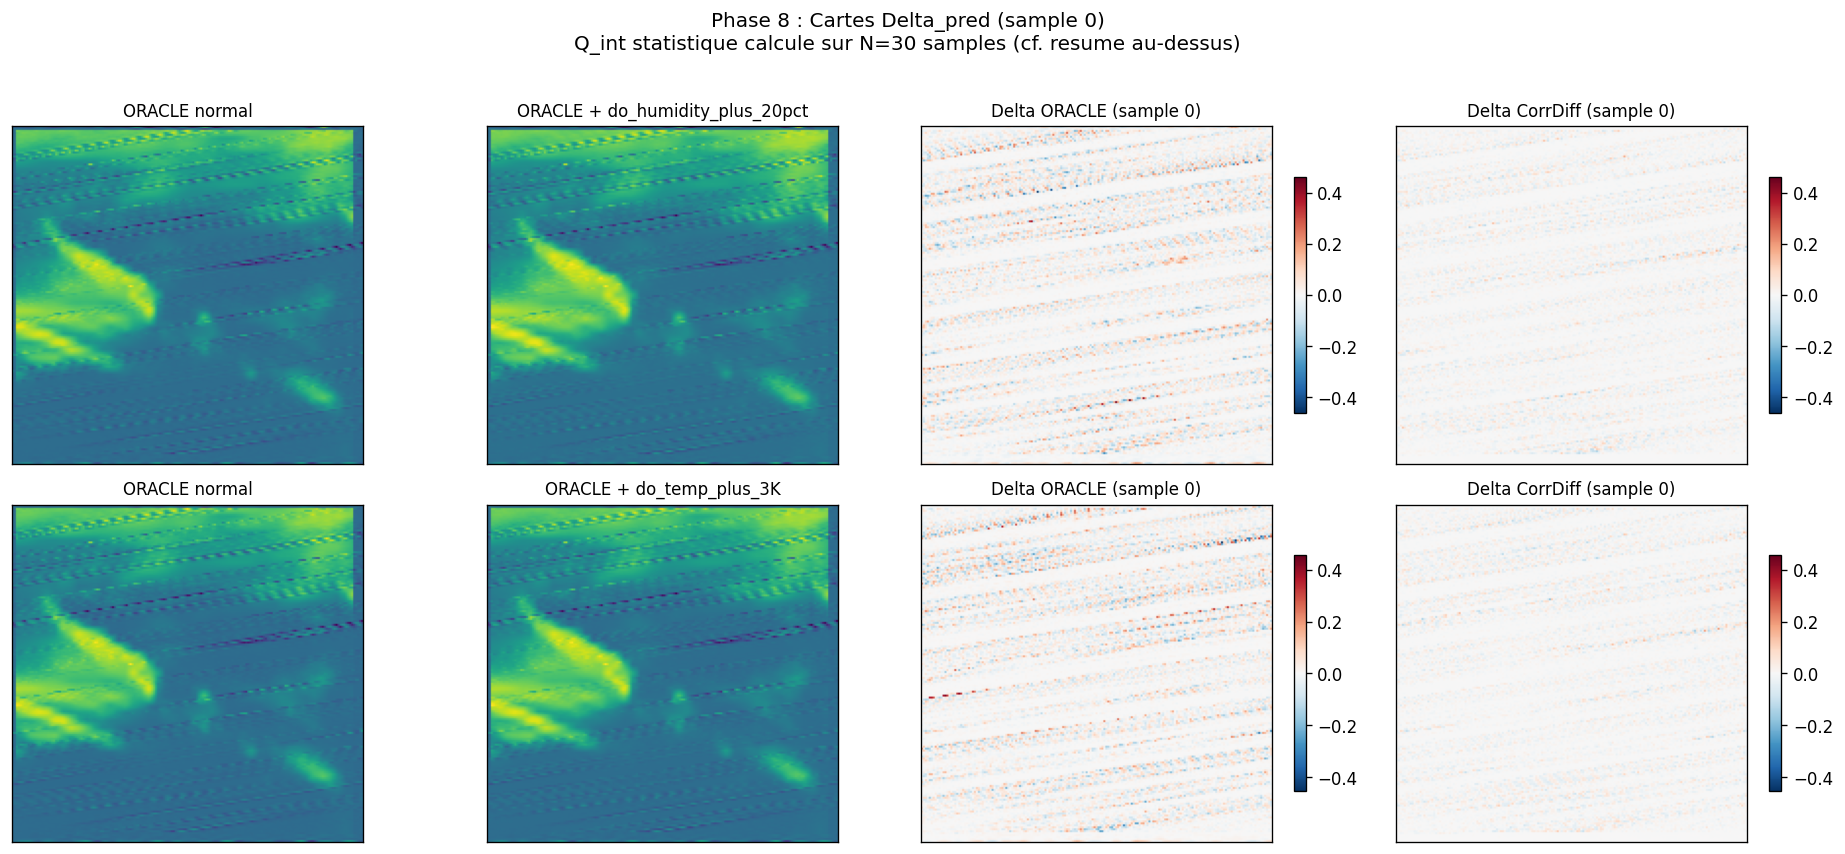
\includegraphics[width=0.85\linewidth]{../results/v5_evaluation/phase8_figures/03_interventions_maps.png}
\caption{Cartes des perturbations contrôlées $\Delta q+20\%$ et $\Delta t+3$~K. Signes physiques cohérents avec la relation de Clausius-Clapeyron sur les deux perturbations testées.}
\label{fig:exp-interventions}
\end{figure}

\begin{figure}[H]
\centering
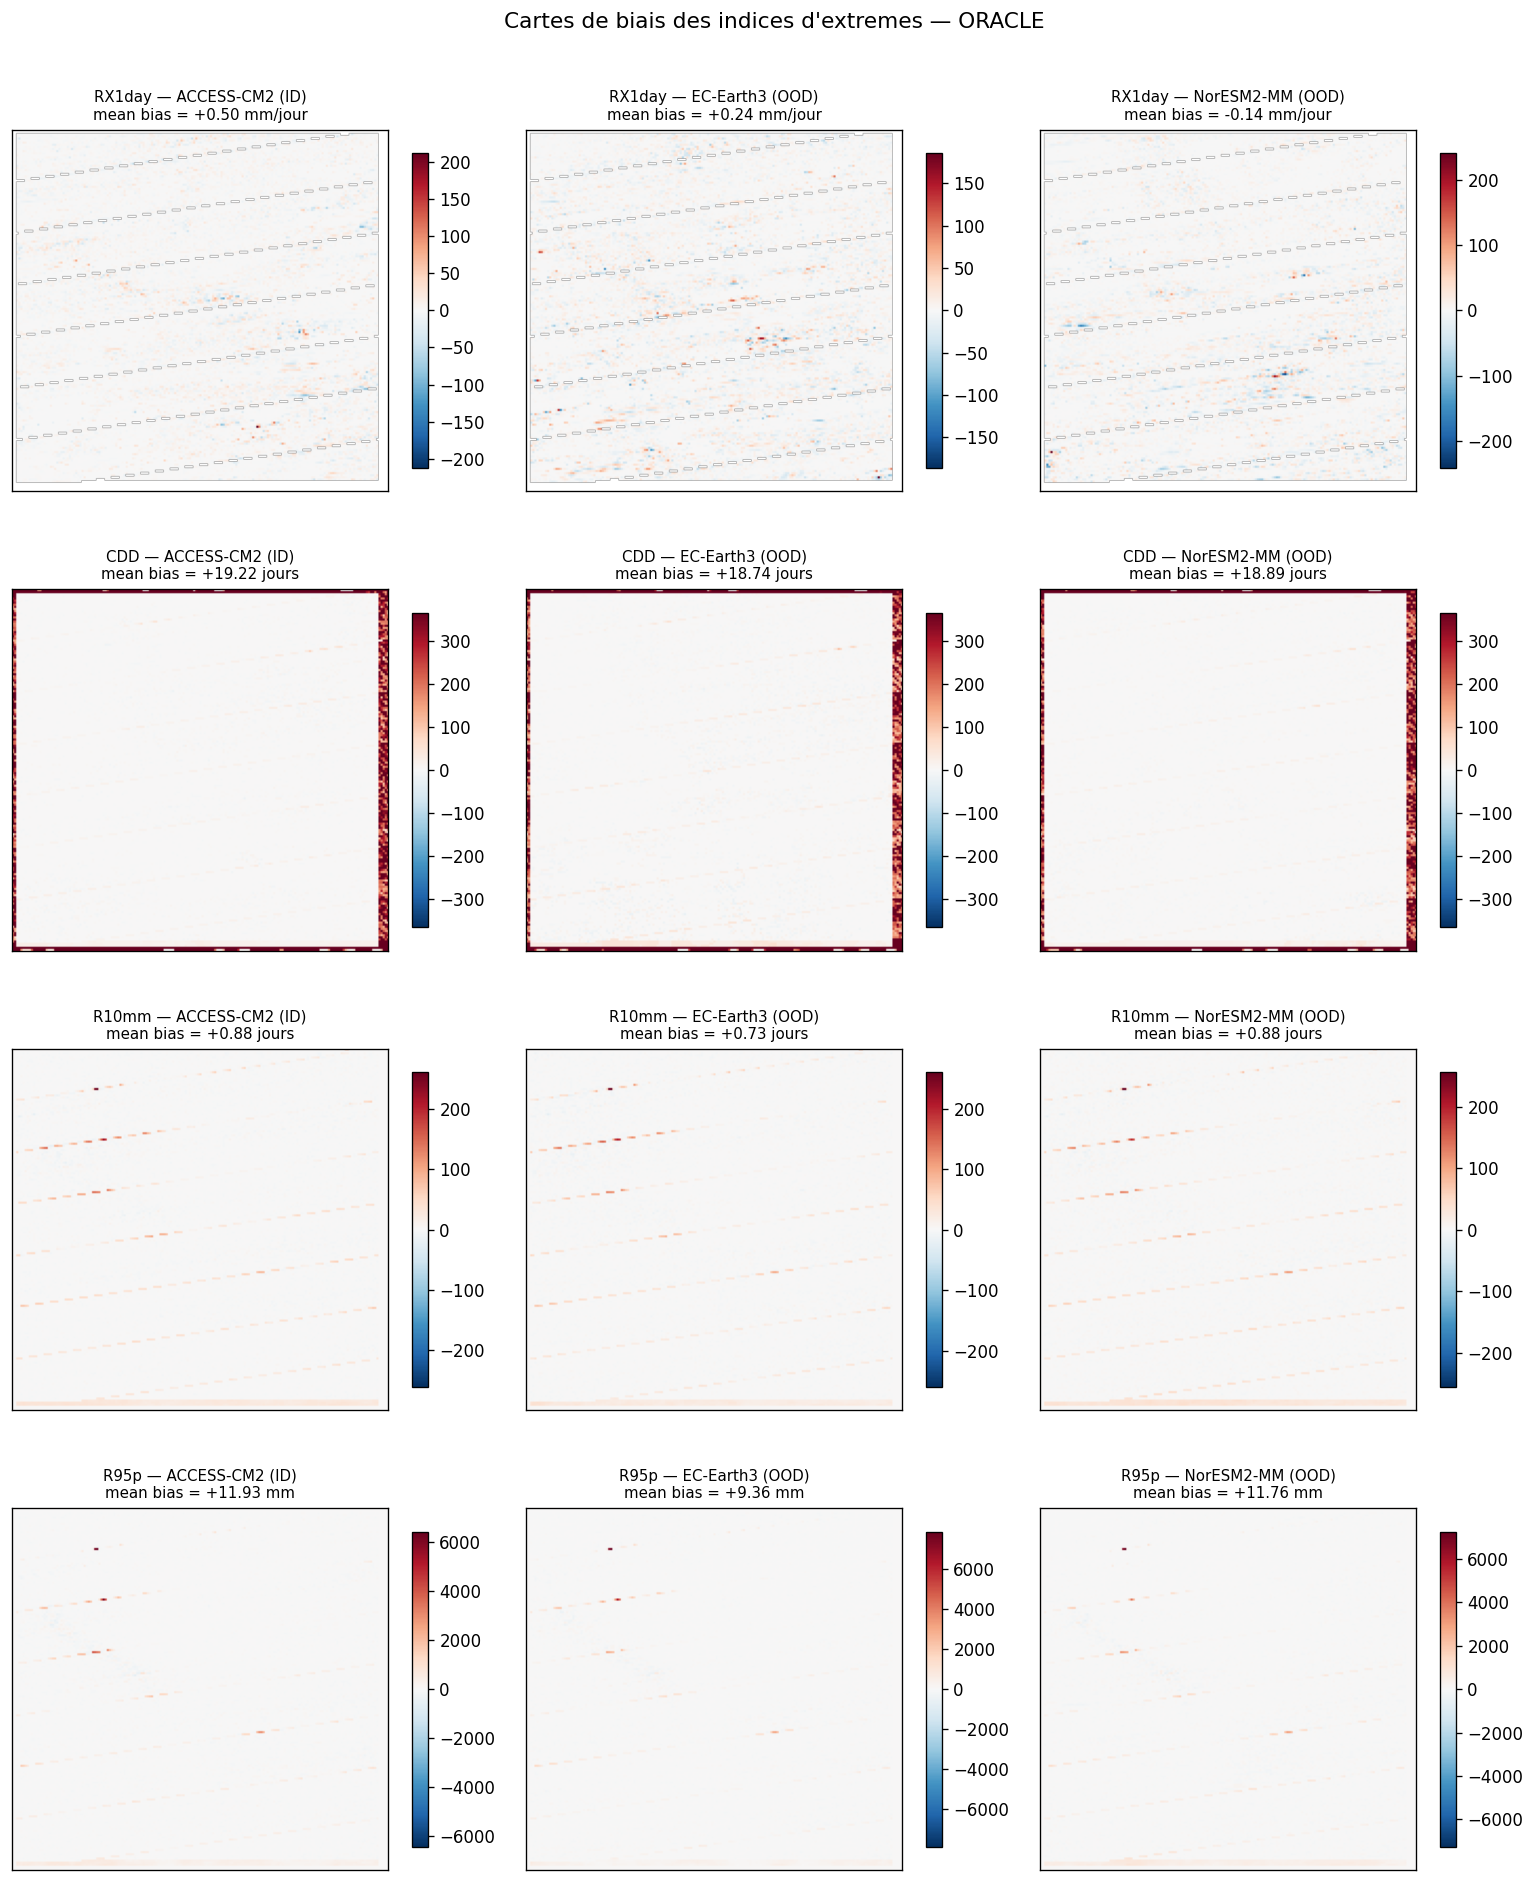
\includegraphics[width=0.78\linewidth]{../results/v5_evaluation/phase10_extreme_bias_maps/extreme_bias_ORACLE.png}
\caption{Biais sur l'indice RX1day pour \Oracle{}. Le déficit, concentré sur le versant occidental des Southern Alps, révèle l'absence d'orographie HR (DEM) en entrée --- même schéma spatial sur \CorrDiff{}, donc la cause est l'information manquante, pas la causalisation.}
\label{fig:exp-extreme-bias-oracle}
\end{figure}

\subsection*{Annexe IV.E --- Métriques climato complémentaires}
\label{ssec:exp-annexe-climato}

Diagnostics climato standards : la distribution log-log des intensités confirme que \Oracle{} reproduit la queue droite tandis que \CorrDiff{} coupe à $\sim 30$~mm/j ; le \emph{Fractions Skill Score} indique que \Oracle{} est \emph{skillful} à l'échelle $\sim 30$~km, contre $\sim 80$~km pour \CorrDiff{}. Figures correspondantes disponibles dans \texttt{results/v5\_evaluation/phase9\_climate\_standards/} (omises pour économiser des pages).

\end{document}
